\documentclass[tikz, margin={5cm 0cm 5cm 5cm}]{standalone}
\usetikzlibrary{lindenmayersystems}
\begin{document}
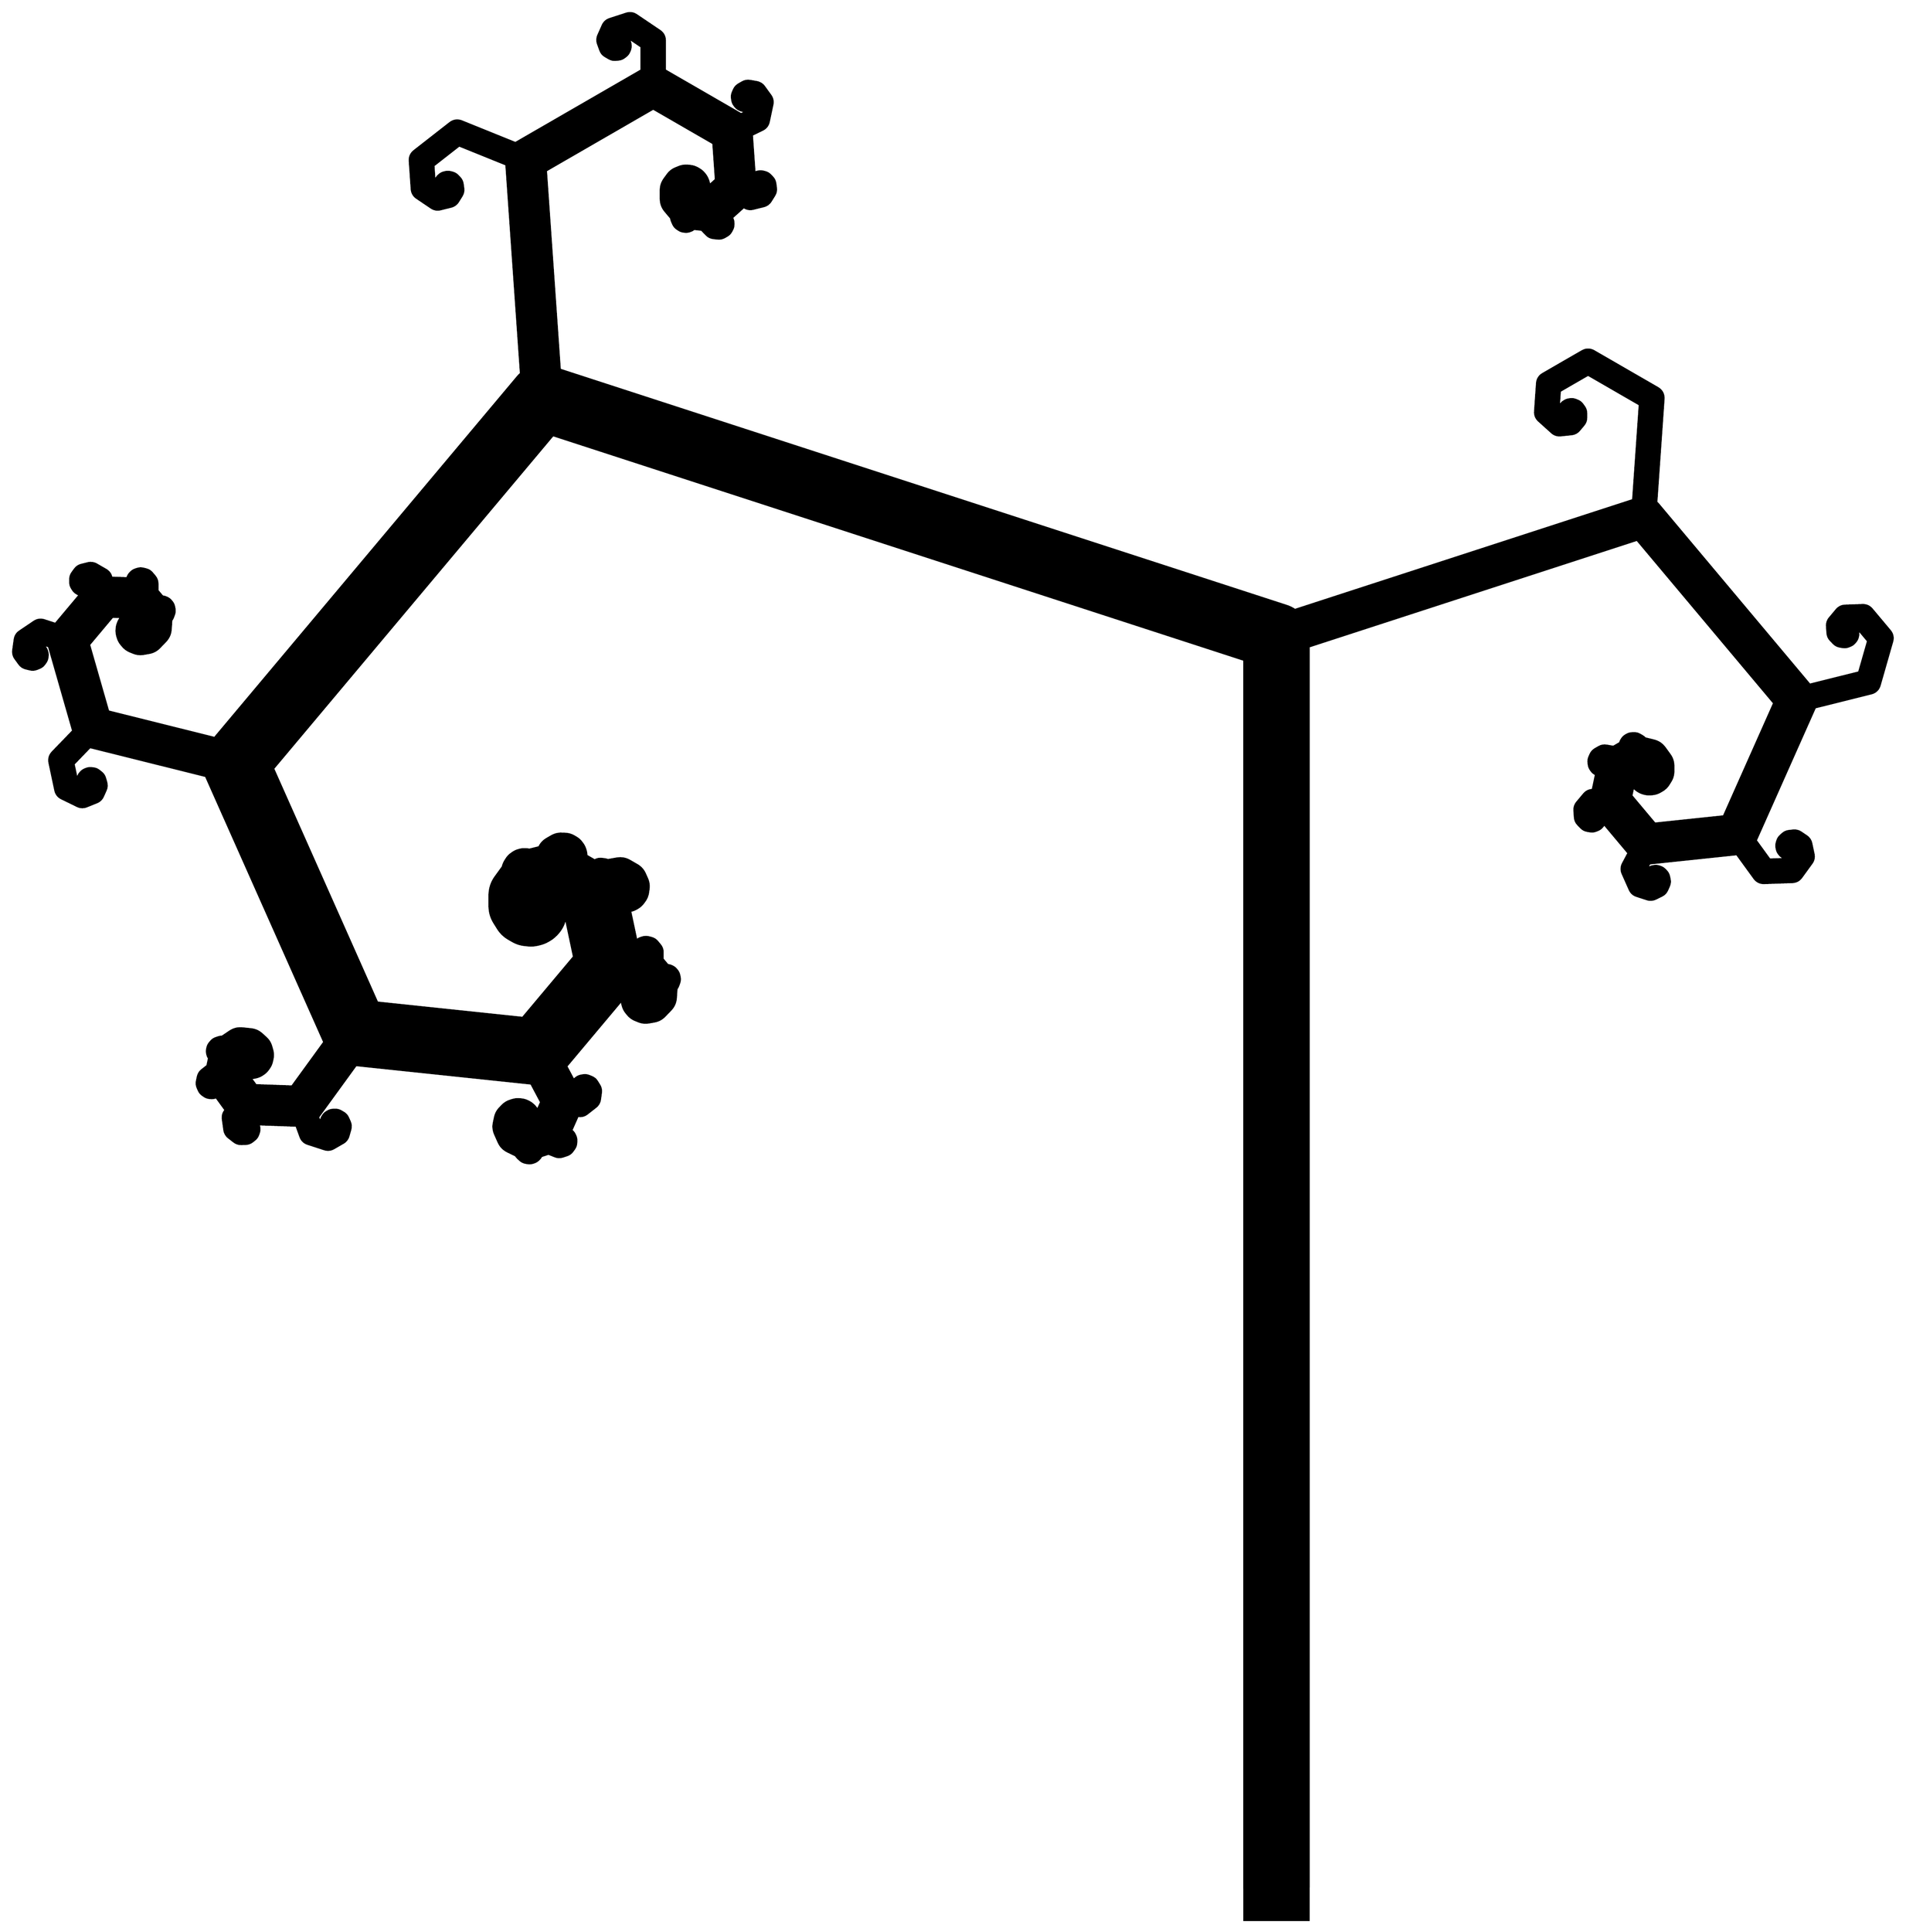
\begin{tikzpicture}
    \tikzset{stab line/.style={cap=round, line join=round,}}
    \pgfdeclarelindenmayersystem{krummstab}{
        % The fact that these \draw commands actually affect the styling is a
        % hack I came across accidentally. I'm not sure how and why it works.
        \symbol{F}{\draw[stab line, line width=55pt];\pgflsystemdrawforward}
        \symbol{A}{\draw[stab line, line width=34pt];\pgflsystemdrawforward}
        \symbol{R}{\draw[stab line, line width=21pt];\pgflsystemdrawforward}
        \symbol{L}{\pgflsystemdrawforward}
        \symbol{B}{\pgflsystemdrawforward}
        \symbol{S}{\pgflsystemdrawforward}
        \rule{F -> LLLL[+MF][-NA]}
        \rule{M -> +M}
        \rule{O -> ++O}
        \rule{N -> -N}
        \rule{L -> LX}
        \rule{X -> L}
        \rule{A -> BB[-NA][+MR]}
        \rule{B -> BY}
        \rule{Y -> B}
        \rule{R -> S[+MR]}
        \rule{S -> ST}
        \rule{T -> S}
    }
    \draw[black, rotate=90] lindenmayer system[lindenmayer system={krummstab,
        step=.1pt, angle=4, axiom=F, order=18}];
    % This last line just ensures that the round cap at the bottom of the staff
    % is not visible.
    \draw[overlay, black, line width=55pt] (0, 0) -- (0, -1);
\end{tikzpicture}
\end{document}
